
%(BEGIN_QUESTION)
% Copyright 2015, Tony R. Kuphaldt, released under the Creative Commons Attribution License (v 1.0)
% This means you may do almost anything with this work of mine, so long as you give me proper credit

Suppose we have a PLC connected to two process switches as shown in this illustration:

$$\includegraphics[width=15.5cm]{i01879x01.eps}$$

Based on the highlighting you see in the ``live'' PLC program display, determine as best you can the pressure and temperature stimulating each switch:

\vskip 20pt \vbox{\hrule \hbox{\strut \vrule{} {\bf Suggestions for Socratic discussion} \vrule} \hrule}

\begin{itemize}
\item{} Identify which LED indicators on the PLC's face would be lit in this condition.
\end{itemize}

\underbar{file i01879}
%(END_QUESTION)





%(BEGIN_ANSWER)


%(END_ANSWER)





%(BEGIN_NOTES)

Based on the color highlighting, we can see that every contact instruction linked to bits {\tt X1} and {\tt X3} are in their ``resting'' states, which means bits {\tt X1} and {\tt X3} must both be zero (0).  All contact instructions linked to bit {\tt X5}, however, are in their actuated states which means bit {\tt X5} must be one (1).

This means the switches connected to inputs {\tt X1} and {\tt X3} are open, thus de-energizing those PLC inputs and leaving those bits in the zero state.  Conversely, the switch connected to input {\tt X5} is closed, energizing that PLC input and setting that bit to the one state.

Any process switch in its resting state must be experiencing a stimulus below its trip point.  Any process switch in its actuated state must be experiencing a stimulus above its trip point.  Thus, we may determine process stimuli as follows:

\vskip 10pt

\noindent
We know the level switch is open (in order to yield an {\tt X1} bit state of zero (0), and it is wired normally-open.  This means that switch must be at rest, with a level condition {\it less than 3 feet}.

\vskip 10pt

\noindent
We know the pressure switch is open (in order to yield an {\tt X3} bit state of zero (0), and it is wired normally-closed.  This means that switch must be actuated, with a pressure condition {\it greater than 25 PSI}.

\vskip 10pt

\noindent
We know the temperature switch is closed (in order to yield an {\tt X5} bit state of one (1), and it is wired normally-open.  This means that switch must be actuated, with a temperature condition {\it greater than 170 $^{o}$F}.













\vfil \eject

\noindent
{\bf Prep Quiz:}

Determine the actuation statuses of the pushbuttons in this PLC system (i.e. pressed versus unpressed), given the live status highlighting shown in the PLC program:

$$\includegraphics[width=15.5cm]{i01879x02.eps}$$

\vfil \eject

\noindent
{\bf Prep Quiz:}

Determine the actuation statuses of the pushbuttons in this PLC system (i.e. pressed versus unpressed), given the live status highlighting shown in the PLC program:

$$\includegraphics[width=15.5cm]{i01879x03.eps}$$

\vfil \eject

\noindent
{\bf Prep Quiz:}

Determine the actuation statuses of the pushbuttons in this PLC system (i.e. pressed versus unpressed), given the live status highlighting shown in the PLC program:

$$\includegraphics[width=15.5cm]{i01879x04.eps}$$




%INDEX% PLC, relating I/O status to virtual elements 

%(END_NOTES)


